% !TEX root = ../OT4ML.tex

\section{Beyond Comparing Measures}
\label{sec-beyond-comparing-measures}

The last group leaves the setting of scalar measures on a common ambient space. Vector and tensor-valued OT transports matrix-valued mass with internal degrees of freedom, Gromov--Wasserstein compares metric-measure spaces without a prescribed correspondence, and quantum OT replaces scalar couplings by positive operators. In each case, the transport plan also has to encode structure carried by the support, the fibers or the non-commutative state space.

\subsection{Vector and Tensor-Valued Measures}
\label{sec-vector-tensor-valued-measures}

Scalar OT transports a nonnegative density. In imaging, diffusion tensor imaging, spectral analysis and quantum-inspired models, the mass attached to a point can instead be a vector, a covariance matrix or a positive semidefinite tensor. A convenient finite-dimensional model is a matrix-valued measure $A$ on $\X$ with values in $\mathbb H_m^+$, the cone of $m\times m$ positive semidefinite Hermitian matrices. If $A$ has a density, we write $A(x)\succeq0$ and interpret $\tr A(x)$ as the local amount of mass while the normalized matrix describes an internal state. Static matrix-valued Monge--Kantorovich problems and dual test-function metrics were developed in~\cite{Ning2014metrics,JiangSpectral,ning2015matrix}; dynamic non-commutative versions are closely related to the matrix transport models of~\cite{Chen2016,ChenGangbo17} and to non-commutative Wasserstein geometries for density matrices~\cite{Carlen2014,2016-peyre-qot}.

A Benamou--Brenier-type construction introduces, in addition to the matrix density $A_t(x)$, a spatial matrix flux $M_t(x)=(M_{t,1},\ldots,M_{t,d})$ and sometimes an internal flux $Q_t(x)=(Q_{t,r})_r$ that rotates or mixes the matrix fibers. A schematic matrix-perspective action, written in the simplest left-perspective convention, is
\begin{equation}\label{eq-matrix-valued-bb}
\begin{aligned}
\mathcal W_{\mathrm{mv}}^2(A_0,A_1)
=\inf_{A,M,Q}\int_0^1\!\int_\X
\Bigg[
\sum_{\ell=1}^d \tr\big(M_{t,\ell}^* A_t^\dagger M_{t,\ell}\big)
+\lambda\sum_r \tr\big(Q_{t,r}^* A_t^\dagger Q_{t,r}\big)
\Bigg]\d x\d t
\end{aligned}
\end{equation}
subject to the endpoint constraints and to a continuity equation
\begin{equation}\label{eq-matrix-valued-continuity}
\partial_t A_t+\nabla_x\cdot M_t+\nabla_L^* Q_t=0.
\end{equation}
Here $A^\dagger$ denotes the Moore--Penrose inverse, with the usual perspective convention: the action is finite only when the fluxes are supported in the range of $A$. In genuinely non-commutative settings, one often replaces the displayed left-perspective expression by a symmetrized left-right perspective; this choice is part of the definition of the metric and is what ensures convexity and compatibility with adjoints. The operator $\nabla_L$ is a non-commutative gradient generated by a finite family of matrices $(L_r)_r$, for instance $\nabla_L X=(L_rX-XL_r)_r$, and $\nabla_L^*$ is its adjoint. The spatial term moves matrix-valued mass through $\X$; the internal term changes the fiber state without spatial displacement. If $m=1$ and $Q=0$,~\eqref{eq-matrix-valued-bb} reduces to the scalar Benamou--Brenier action of Section~\ref{sec-dynamic-optimal-transport}. If $\X$ is a single point, only the internal non-commutative transport remains, giving a dynamic geometry on positive matrices.

The important point is not the particular choice of $\nabla_L$, but the variational grammar. One chooses admissible spatial and internal directions, writes a linear continuity equation for the matrix density, and minimizes a convex matrix-perspective kinetic energy. Different choices of $L_r$, symmetrization conventions and boundary conditions give different tensor-valued Wasserstein metrics. These models are useful when the transported object carries orientation, color covariance, spectral content or a quantum state, and they provide the dynamic counterpart of the finite-dimensional quantum couplings described below.


\subsection{Gromov--Wasserstein}
\label{sec-gromov-wasserstein}

Gromov--Wasserstein compares spaces through their internal distance structures rather than through a fixed ambient ground cost. This is the right extension for graphs, shapes and point clouds whose points are not pre-aligned.

\paragraph{Discrete formulation.}

Optimal transport needs a ground cost $\C$ to compare histograms $(\a,\b)$, and thus cannot be used directly if the histograms are not defined on the same underlying space, or if one cannot pre-register these spaces to define a ground cost.
%
To address this issue, one can instead use a weaker requirement: two matrices $\distD \in \RR^{n \times n}$ and $\distD' \in \RR^{m \times m}$ are available and represent relationships between the points on which the histograms are defined. A typical scenario is when these matrices are powers of distance matrices.
%
The Gromov--Wasserstein problem reads
\eql{\label{eq-gw-def}
	\GWD( (\a,\distD), (\b,\distD') )^p \eqdef
	\umin{ \P \in \CouplingsD(\a,\b) }
		\Ee_{\distD,\distD'}(\P) \eqdef
		\sum_{i,j,i',j'} \De(\distD_{i,i'},\distD'_{j,j'})^p \P_{i,j}\P_{i',j'},
}
where $p \geq 1$ and $\De$ is a distance on $\RR$, typically $\De(u,v)=|u-v|$.
%
This is a non-convex quadratic problem over the transport polytope. In the uniform case with the additional hard-assignment constraint $m=n$ and $\P$ a permutation matrix, it becomes a Quadratic Assignment Problem (QAP)~\cite{loiola-2007}; this restricted graph-matching form is already NP-hard in full generality.
%
The relaxed coupling formulation used in GW can therefore be read as a soft graph-matching model~\cite{lyzinski-2015}.

\begin{figure}[ht]
\centering
\begin{tabular}{@{}ccc@{}}
\small isometric copy &
\small mild deformation &
\small strong deformation \\[-.15em]

\includegraphics[width=.30\linewidth]{figures/gromov-isometry-matching/isometric.pdf} &
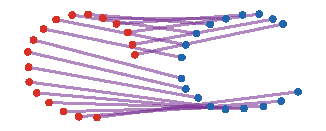
\includegraphics[width=.30\linewidth]{figures/gromov-isometry-matching/mild-deformation.pdf} &
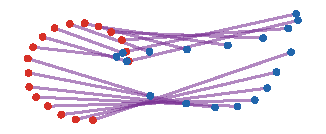
\includegraphics[width=.30\linewidth]{figures/gromov-isometry-matching/strong-deformation.pdf}
\end{tabular}
\caption{Gromov--Wasserstein correspondences under increasing deformation. The red and blue point clouds are not compared through an ambient Euclidean cross-cost; instead, the GW coupling compares their internal pairwise distances. A perfectly isometric copy admits a clean structural match, while mild and strong deformations progressively bend the correspondence.}
\label{fig:gromov-isometry-matching}
\end{figure}

When the matrices $\distD,\distD'$ are genuine distance matrices, the general construction below shows that $\GWD$ satisfies the triangle inequality and defines a distance between metric spaces equipped with a probability distribution, up to measure-preserving isometries.
%
This distance was introduced and studied in detail by Memoli in~\cite{memoli-2011}. An in-depth mathematical exposition (in particular, its geodesic structure and gradient flows) is given in~\cite{SturmGW}. See also~\cite{schmitzer2013modelling} for applications in computer vision.
%
Its relation to Hausdorff and Gromov--Hausdorff distances is discussed at the end of this subsection.

%%%%%%%%%%%%%%%%%%%%%
\paragraph{General setting.}

The general setting corresponds to computing couplings between metric measure spaces $\XX=(\X,\dist_\X,\al)$
	and $\YY=(\Y,\dist_\Y,\be)$ where $(\dist_\X,\dist_\Y)$ are distances and $(\al,\be)$ are measures on their respective spaces.
	%
	The natural setting is that of Polish metric spaces; compactness is often assumed in this section to avoid existence and integrability issues.
	%
	One defines
	\begin{align}
		\label{eq-gw-generic}
		\GW( \XX,\YY )^p \eqdef
		\umin{ \pi \in \Couplings(\al,\be) }
		\int_{\X^2 \times \Y^2}
		 \De(\dist_\X(x,x'),\dist_\Y(y,y'))^p
		\d\pi(x,y)\d\pi(x',y').
	\end{align}

\begin{prop}[Euclidean GW is controlled by Wasserstein]\label{prop-gw-controlled-by-wasserstein}
	Let $\alpha,\beta$ be probability measures on $\RR^d$, equipped with the Euclidean distance, and take $\De(u,v)=|u-v|$ in~\eqref{eq-gw-generic}. Then
	\[
		\GW((\RR^d,\norm{\cdot},\alpha),(\RR^d,\norm{\cdot},\beta))
		\leq
		2\Wass_p(\alpha,\beta).
	\]
\end{prop}
\begin{proof}
	Let $\pi$ be any coupling between $\alpha$ and $\beta$. For two independent pairs $(X,Y),(X',Y')\sim\pi$, the reverse triangle inequality gives
	\[
		\big|\norm{X-X'}-\norm{Y-Y'}\big|
		\leq
		\norm{X-Y}+\norm{X'-Y'}.
	\]
	Taking the $L^p$ norm and using Minkowski gives a bound by $2(\int\norm{x-y}^p\d\pi)^{1/p}$. Optimizing over $\pi$ proves the claim.
\end{proof}

In the following, one says that $\XX$ and $\YY$ are isometric mm-spaces if there exists $\phi : \X \rightarrow \Y$ such that $\phi_{\sharp}\al=\be$ and which is a bijective isometry between the supports of $\al$ and $\be$, i.e. $\dist_\Y(\phi(x),\phi(x'))=\dist_\X(x,x')$ on the support of $\al$.

\begin{figure}[ht]
\centering
\begin{tabular}{@{}cc@{}}
\small correspondence &
\small pairwise-distance residual \\[-.15em]

\includegraphics[width=.43\linewidth]{figures/gromov-nonisometric-distortion/correspondence.pdf} &
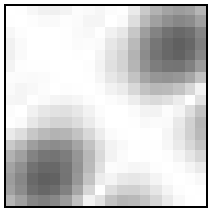
\includegraphics[width=.23\linewidth]{figures/gromov-nonisometric-distortion/distance-residual.pdf}
\end{tabular}
\caption{Local distortion in a non-isometric GW match. The left panel colors transport segments by the average residual induced by the displayed hard correspondence. The right panel shows the pairwise-distance residual matrix $|d_\X(x_i,x_{i'})-d_\Y(y_{\sigma(i)},y_{\sigma(i')})|$, which is the local contribution minimized by the discrete GW objective for this correspondence.}
\label{fig:gromov-nonisometric-distortion}
\end{figure}

\paragraph{Adding features.}
Fused Gromov--Wasserstein augments the structural term with a feature transport cost. In the discrete case, given a cross-feature cost $M\in\RR^{n\times m}$ and a parameter $\eta\in[0,1]$, one minimizes
\[
	\umin{\P\in\CouplingsD(\a,\b)}
	(1-\eta)\sum_{i,j}M_{ij}\P_{ij}
	+\eta
	\sum_{i,j,i',j'}\De(\distD_{ii'},\distD'_{jj'})^p\P_{ij}\P_{i'j'}.
\]
The first term compares node attributes in the usual OT sense, while the second compares the intrinsic geometry. The endpoints $\eta=0$ and $\eta=1$ recover feature-only OT and pure GW respectively; intermediate values trade attribute matching against structural matching. This is useful when the two spaces have both distances and features, and these two sources of information may disagree.

\begin{figure}[ht]
\centering
\begin{tabular}{@{}ccc@{}}
\small feature-only OT &
\small fused GW &
\small pure GW \\[-.15em]

\includegraphics[width=.30\linewidth]{figures/fused-gromov-feature-geometry/feature-ot.pdf} &

\includegraphics[width=.30\linewidth]{figures/fused-gromov-feature-geometry/fused-gw.pdf} &

\includegraphics[width=.30\linewidth]{figures/fused-gromov-feature-geometry/pure-gw.pdf}
\end{tabular}
\caption{Feature information and intrinsic geometry in fused Gromov--Wasserstein. Small inner disks encode binary node features. Feature-only OT follows the attributes even when this crosses the shape structure, pure GW follows the intrinsic ordering, and fused GW balances the feature term with the pairwise-distance distortion.}
\label{fig:fused-gromov-feature-geometry}
\end{figure}

\subsection{Quantum Optimal Transport}
\label{sec-quantum-ot}

Quantum OT replaces scalar probability vectors by density matrices. In finite dimension, let $\mathbb H_n$ be the Hermitian matrices and let $\mathbb H_n^{+,1}$ be the positive semidefinite Hermitian matrices with trace one. A coupling between $A\in\mathbb H_n^{+,1}$ and $B\in\mathbb H_m^{+,1}$ is a positive semidefinite matrix $T\in\mathbb H_{nm}^+$ whose partial traces are $A$ and $B$:
\begin{equation}\label{eq-qot-partial-traces}
	\operatorname{Tr}_B(T)=A,
	\qquad
	\operatorname{Tr}_A(T)=B,
\end{equation}
where the partial traces are characterized by
\[
	\tr(F\,\operatorname{Tr}_B T)=\tr((F\otimes\Id_m)T),
	\qquad
	\tr(G\,\operatorname{Tr}_A T)=\tr((\Id_n\otimes G)T)
\]
for all $F\in\mathbb H_n$ and $G\in\mathbb H_m$.
Given a Hermitian cost observable $C\in\mathbb H_{nm}$, the finite-dimensional quantum OT problem is the semidefinite program
\begin{equation}\label{eq-qot-primal}
	\mathrm{QOT}_C(A,B)
	\eqdef
	\min_{T\succeq0}
	\enscond{\tr(CT)}{\operatorname{Tr}_B(T)=A,\ \operatorname{Tr}_A(T)=B}.
\end{equation}
This is the direct non-commutative analogue of a Kantorovich coupling: nonnegativity becomes positive semidefiniteness and marginal constraints become partial-trace constraints.


\begin{prop}[Quantum Kantorovich duality]\label{prop-qot-duality}
	For $A\in\mathbb H_n^{+,1}$ and $B\in\mathbb H_m^{+,1}$, the dual of~\eqref{eq-qot-primal} is
	\begin{equation}\label{eq-qot-dual}
		\mathrm{QOT}_C(A,B)
		=
		\max_{F\in\mathbb H_n,\ G\in\mathbb H_m}
		\left\{
			\tr(FA)+\tr(GB)
			:\,
			F\otimes\Id_m+\Id_n\otimes G\preceq C
		\right\}.
	\end{equation}
	If $A$ and $B$ are positive definite, strong duality follows directly from Slater's condition; the semidefinite case follows by restriction to the supports of $A$ and $B$ or by approximation.
\end{prop}

\begin{proof}
	Introduce Hermitian Lagrange multipliers $F$ and $G$ for the two marginal constraints. The Lagrangian is
	\[
		\tr(CT)+\tr\!\left(F(A-\operatorname{Tr}_B T)\right)
		+\tr\!\left(G(B-\operatorname{Tr}_A T)\right)
		=
		\tr(FA)+\tr(GB)
		+\tr\!\left((C-F\otimes\Id_m-\Id_n\otimes G)T\right),
	\]
	where~\eqref{eq-qot-partial-traces} was used in the last equality. Minimizing over $T\succeq0$ gives a finite lower bound if and only if $C-F\otimes\Id_m-\Id_n\otimes G\succeq0$, in which case the infimum in $T$ is $0$. This gives the dual program. When $A,B\succ0$, the coupling $A\otimes B$ is strictly feasible, so Slater's theorem gives equality of primal and dual values and dual attainment. The general finite-dimensional semidefinite case is obtained by approximation $A_\delta=(1-\delta)A+\delta\Id_n/n$, $B_\delta=(1-\delta)B+\delta\Id_m/m$ and by compactness, or equivalently by reducing to the supports of $A$ and $B$.
\end{proof}

The dual potentials have the usual scalar gauge freedom: replacing $(F,G)$ by $(F+t\Id_n,G-t\Id_m)$ leaves both the constraint and the value unchanged because $\tr(A)=\tr(B)=1$.

\paragraph{Entropic regularization and Bregman iterations.}
As in scalar OT, one obtains a smoother problem by adding the von~Neumann entropy
\[
	H(T)=\tr\!\left(T(\log T-\Id_{nm})\right),
	\qquad
	\nabla H(T)=\log T,
\]
with the convention $0\log0=0$. For $\epsilon>0$ define
\begin{equation}\label{eq-qot-entropic-primal}
	\mathrm{QOT}_C^\epsilon(A,B)
	=
	\min_{T\succeq0}
	\left\{
		\tr(CT)+\epsilon H(T)
		:\,
		\operatorname{Tr}_B(T)=A,
		\operatorname{Tr}_A(T)=B
	\right\}.
\end{equation}
This is the non-commutative analogue of entropic OT~\cite{2016-peyre-qot,chakrabarti2019quantum}: the Shannon entropy of a coupling is replaced by the trace entropy of a density matrix.

\begin{prop}[Entropic quantum OT duality]\label{prop-qot-entropic-duality}
	Assume $A\succ0$, $B\succ0$ and $\epsilon>0$. Then~\eqref{eq-qot-entropic-primal} has a unique positive minimizer. Its dual is
	\begin{equation}\label{eq-qot-entropic-dual}
		\mathrm{QOT}_C^\epsilon(A,B)
		=
		\max_{F\in\mathbb H_n,\ G\in\mathbb H_m}
		\left\{
			\tr(FA)+\tr(GB)
			-\epsilon\,
			\tr\exp\!\left(\frac{F\otimes\Id_m+\Id_n\otimes G-C}{\epsilon}\right)
		\right\}.
	\end{equation}
	At optimality, primal and dual variables are linked by the Gibbs formula
	\begin{equation}\label{eq-qot-gibbs-coupling}
		T_e(F,G)
		=
		\exp\!\left(\frac{F\otimes\Id_m+\Id_n\otimes G-C}{\epsilon}\right),
	\end{equation}
	with $\operatorname{Tr}_B(T_e)=A$ and $\operatorname{Tr}_A(T_e)=B$.
\end{prop}

\begin{proof}
	The feasible set is compact and nonempty, and it contains the positive definite point $A\otimes B$. The trace entropy is strictly convex on positive semidefinite matrices, hence the regularized primal has a unique minimizer. Slater's condition justifies the Lagrange dual computation. The Fenchel identity
	\[
		\sup_{T\succeq0}\ \tr(YT)-\epsilon H(T)
		=
		\epsilon\,\tr\exp(Y/\epsilon)
	\]
	is the matrix analogue of the scalar exponential conjugacy. Applying it to the Lagrangian of~\eqref{eq-qot-entropic-primal}, with
	$Y=F\otimes\Id_m+\Id_n\otimes G-C$, gives~\eqref{eq-qot-entropic-dual}. The stationarity condition of this Fenchel identity gives~\eqref{eq-qot-gibbs-coupling}; differentiating the dual objective with respect to $F$ and $G$ yields the two marginal equations.
\end{proof}

Writing $K=\exp(-C/\epsilon)$, the objective in~\eqref{eq-qot-entropic-primal} differs by a constant from $\epsilon$ times the quantum KL divergence
\[
	D_H(T|K)
	=
	\tr\!\left(T(\log T-\log K)-T+K\right).
\]
The exact quantum analogue of Sinkhorn is an implicit alternating Bregman projection scheme onto the affine marginal sets
\[
	\mathcal M_A=\{T\succeq0:\operatorname{Tr}_B(T)=A\},
	\qquad
	\mathcal M_B=\{T\succeq0:\operatorname{Tr}_A(T)=B\}.
\]

\begin{prop}[Exact Bregman projections]\label{prop-qot-bregman-projections}
	Assume $A,B\succ0$ and let $K=\exp(-C/\epsilon)$. The minimizer of~\eqref{eq-qot-entropic-primal} is equivalently the minimizer of $D_H(T|K)$ over $\mathcal M_A\cap\mathcal M_B$. Moreover, if a current positive definite matrix has Gibbs form $T_e(F,G)$, then its Bregman projection onto $\mathcal M_A$ has the form $T_e(F^+,G)$, where $F^+$ is chosen so that $\operatorname{Tr}_B T_e(F^+,G)=A$. The projection onto $\mathcal M_B$ is analogous. Thus, when each one-block marginal equation is solved exactly, alternating Bregman projections are equivalent to alternating block maximization of the dual~\eqref{eq-qot-entropic-dual}.
\end{prop}

\begin{proof}
	Since $\log K=-C/\epsilon$, the identity
	\[
		\tr(CT)+\epsilon H(T)
		=
		\epsilon D_H(T|K)-\epsilon\tr(K)
	\]
	holds, so the primal minimizer is the constrained Bregman projection of $K$ up to an additive constant. For the projection of a positive definite matrix $S$ onto $\mathcal M_A$, the affine set contains the positive definite point $A\otimes\Id_m/m$; the entropy derivative $\log T-\log S$ is singular at the boundary, so the projection lies in the interior of the positive cone. Its Lagrangian first variation is
	\[
		\log T-\log S-\Lambda\otimes\Id_m=0
	\]
	for a Hermitian multiplier $\Lambda$. Hence $T=\exp(\log S+\Lambda\otimes\Id_m)$. If $S=T_e(F,G)$, this is again of the form $T_e(F+\epsilon\Lambda,G)$. The multiplier is fixed by the marginal equation $\operatorname{Tr}_B(T)=A$. The same argument applies to $\mathcal M_B$. Finally, the first-order optimality condition for maximizing~\eqref{eq-qot-entropic-dual} over one block is exactly the corresponding marginal equation, so the Bregman and block-dual views coincide.
\end{proof}

In the diagonal case this proposition gives the usual multiplicative Sinkhorn updates. In the non-commutative case, however, the exact block equations
\[
	\operatorname{Tr}_B T_e(F,G)=A,
	\qquad
	\operatorname{Tr}_A T_e(F,G)=B
\]
do not admit scalar division formulas, because the exponential of $F\otimes\Id_m+\Id_n\otimes G-C$ cannot be separated unless the local potential $F\otimes\Id_m+\Id_n\otimes G$ commutes with the cost $C$.
When all matrices are diagonal in the same basis, commutativity restores the scalar form $T_e=\diag(u)K\diag(v)$ and the marginal equations reduce to the usual Sinkhorn divisions.

\paragraph{Gurvits scaling and quantum Sinkhorn.}
The algorithm often called quantum Sinkhorn comes from the operator-scaling literature of Gurvits and subsequent developments~\cite{gurvits2003classical,gurvits2004classical,georgiou2015positive,garg2018recent}. It replaces the true Gibbs coupling~\eqref{eq-qot-gibbs-coupling} by the symmetric factorization
\begin{equation}\label{eq-qot-symmetric-scaling}
	T_s(F,G)
	=
	\exp\!\left(\frac{Z}{2\epsilon}\right)\exp(-C/\epsilon)\exp\!\left(\frac{Z}{2\epsilon}\right)
	=
	(U\otimes V)K(U\otimes V),
	\qquad
	Z=F\otimes\Id_m+\Id_n\otimes G,
\end{equation}
where $U=\exp(F/(2\epsilon))$, $V=\exp(G/(2\epsilon))$ and $K=\exp(-C/\epsilon)$. If $[Z,C]=0$, then $T_s(F,G)=T_e(F,G)$; otherwise this is a Strang-type symmetric surrogate.

Fix a Choi convention and let $\mathcal K:\mathbb H_m\to\mathbb H_n$ be the completely positive map represented by the positive Choi matrix $K$; let $\mathcal K^\star$ be its Hilbert--Schmidt adjoint. Up to the transpose dictated by the chosen Choi convention, the marginal equations for the symmetric coupling take the operator-scaling form
\[
	U\,\mathcal K(V^2)\,U=A,
	\qquad
	V\,\mathcal K^\star(U^2)\,V=B.
\]
They can be enforced by the explicit congruence normalizations
\begin{equation}\label{eq-qot-gurvits-updates}
\begin{aligned}
	R_V&=\mathcal K(V^2),
	&
	U&\leftarrow
	R_V^{-1/2}\bigl(R_V^{1/2} A R_V^{1/2}\bigr)^{1/2}R_V^{-1/2},
	\\
	S_U&=\mathcal K^\star(U^2),
	&
	V&\leftarrow
	S_U^{-1/2}\bigl(S_U^{1/2} B S_U^{1/2}\bigr)^{1/2}S_U^{-1/2}.
\end{aligned}
\end{equation}
These inverse square roots are well-defined when $K\succ0$ and $U,V,A,B\succ0$. This is Gurvits/operator scaling with prescribed targets; when all matrices are diagonal it reduces to classical Sinkhorn scaling, and when the targets are proportional to identities it matches the usual bistochastic operator-scaling normalization, up to the conventional trace normalization.


It is important not to identify~\eqref{eq-qot-gurvits-updates} with the exact Bregman scheme for~\eqref{eq-qot-entropic-primal}. The exact Bregman step would enforce the marginals of $T_e(F,G)=\exp((Z-C)/\epsilon)$ and would be a block maximization of the true concave dual~\eqref{eq-qot-entropic-dual}. Gurvits scaling instead enforces the marginals of the surrogate
\[
	T_s=
	\exp\!\left(\frac{Z}{2\epsilon}\right)
	\exp(-C/\epsilon)
	\exp\!\left(\frac{Z}{2\epsilon}\right).
\]
The two coincide in the commuting/diagonal regime, but in general the Baker--Campbell--Hausdorff commutator terms do not vanish. The Gurvits iteration should therefore be understood as a tractable symmetric operator-scaling approximation to entropic Q--OT, not as the literal alternating KL projection algorithm.

\begin{rem}[Operator-valued couplings]
	The same definitions extend formally from matrices to separable Hilbert spaces by replacing density matrices with positive trace-class operators of trace one, observables with bounded self-adjoint operators and~\eqref{eq-qot-partial-traces} with partial traces defined by duality against local bounded observables. If $\Pi(A,B)$ denotes positive trace-class operators with partial traces $A$ and $B$, a bounded cost observable $C$ gives the problem $\inf_{T\in\Pi(A,B)}\Tr(CT)$. For unbounded positive costs one must define the energy through the quadratic form or spectral truncations, and in the entropic case one must ensure that the Gibbs operator $\exp(-C/\epsilon)$ is trace class and that the partial traces of the candidate coupling are well-defined. The matrix formulas above are therefore the clean finite-dimensional core; the operator version adds domain and compactness assumptions rather than a different algebraic structure.
\end{rem}
